\chapter{Discusión / Análisis de resultados}

\subsection{Análisis de ingeniería} 

Se logra integrar correctamente un sistema mecatrónico capaz de alimentar hasta un total de 30 gallinas. En la imagen \ref{fig:SisAlimEns} se muestra el sistema ensamblado.

\begin{figure}[htbp]
    \centering
    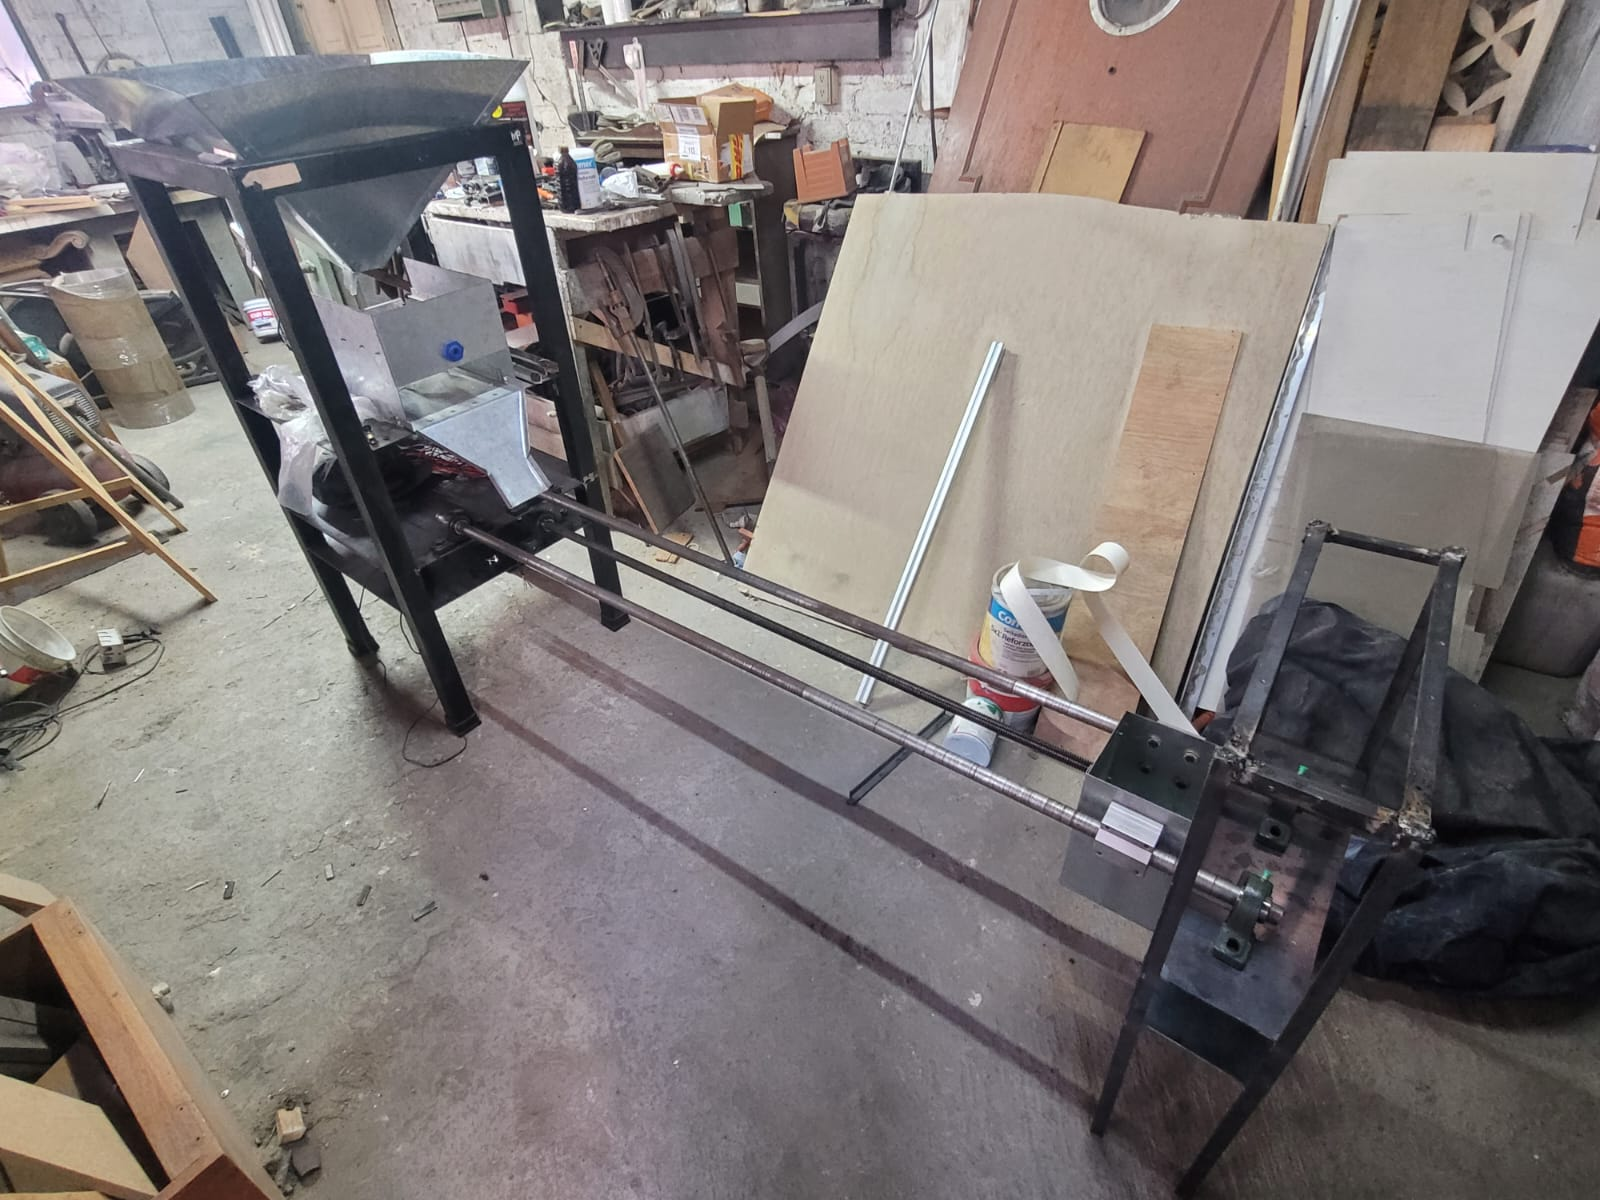
\includegraphics[width=0.75\linewidth]{imagenes/imacap/implementacion/SisFin3.jpeg}
    \caption{Sistema de alimentación ensamblado}
    \label{fig:SisAlimEns}
\end{figure}

Para el diseño del sistema se utilizaron valores superiores a los encontrados en los requerimientos, a fin de tener un factor de seguridad que varía en cada elemento.

Para el caso de las tolvas se detecta un área de mejora al modificar la geometría de ambas, colocando un segmento recto a la salida que permita acoplar de mejor manera y con base a criterios de diseño para el ensamble el mecaniso de apertura y cierre de las mismas.

Se contempla el uso de materiales más ligeros en la fabricación del sistema, como aluminio, que posee una densidad de \SI{7,85}{g/cm}, facilitando así el transporte del sistema.

En el circuito se encuentran problemas en la lectura de los sensores debido al rebote que presentan por ser \textit{switches} mecánicos, los cuales provocan ruido en el sistema.



%\subsection{Análisis de costos} 

%\subsection{Análisis de valor}



%%%%%%fin del archivo
\endinput